\chapter{Modelo proposto}\label{cap:proposta}
Este capítulo abordará o sistema de treinamento proposto. Primeiramente será exposto como funciona todo o ambiente desenvolvido, depois é explicado sobre a configuração dos algoritmos por fim é explicado como será o treinamento e teste dos agentes. 

% Esta seção está sujeita a mudanças feitas no ambiente durante o PGCIII. 
\section{Modelo}\label{modelo}
Aqui é descrito sobre o modelo do projeto. Por "modelo" entende-se o conjunto ambiente-agente-recompensas. Cada um deles é detalhado nas subseções abaixo. Dentre os módulos que compõe um veículo autônomo o foco deste projeto será em desenvolver o componente de controle de deslocamento que é responsável por fazer carro percorrer um trajeto. No mundo real as rotas seriam geradas por outro componente, porém isto está além do escopo deste projeto, portanto elas serão definidas pelo autor. Importante ressaltar que o conjunto de rotas deve ser composto por uma variedade de trajetos que exijam uma diversidade de manobras a serem aprendidas pelo agente.

\subsection{O ambiente}
A simulação envolve em treinar o veículo para percorrer trajetos em ambiente urbano, a princípio, por uma questão de simplicidade o agente não terá de lidar com declives ou aclives, semáforos, outros veículos ou pedestres. Porém outros elementos estáticos comuns de uma cidade como calçadas, postes, árvores, prédios, etc. Portanto, o foco poderá se manter no estudo de fazer um agente percorrer as rotas. Às bordas do cenário há muros que limitam o alcance do veículo, foi concluído pelo autor que o tamanho atual é suficiente para os treinos iniciais, em estudos futuros pode ser considerado a expansão do cenário. O agente recebe uma punição ao se chocar com a calçada ou com os muros da borda da cidade.

\begin{figure}[h]
   \centering
   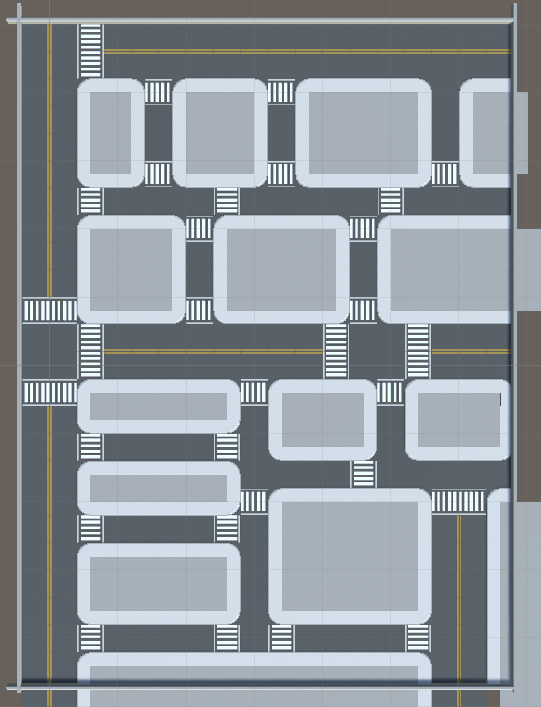
\includegraphics[scale=0.45, angle=90]{figs/Mapa-simulador-visao-superior.png}
    \caption{Visão superior o cenário urbano criado para o treinamento do veículo}
    \label{fig:map-view}
 \end{figure}

As rotas são compostas por: origem, \textit{checkpoints} e destino. O primeiro indica o local de partida do veículo, o último é o objetivo final do agente naquele episódio. Os \textit{checkpoints} são barreiras que indicam o caminho que deve ser percorrido, cada vez que o veículo atravessa uma delas ele ganha uma recompensa, isto é uma forma de indicar a ele que está fazendo o correto. Há 17 percursos predefinidos, cada uma delas possuem características distintas como distância origem-destino, quais e quantas conversões a serem feitas, isto foi moldado visando trazer uma diversidade maior de desafios a serem superados pelo agente. Assim como o tamanho do cenário, novos trajetos podem ser considerados em estudos futuros.

\begin{figure}[h]
   \centering
   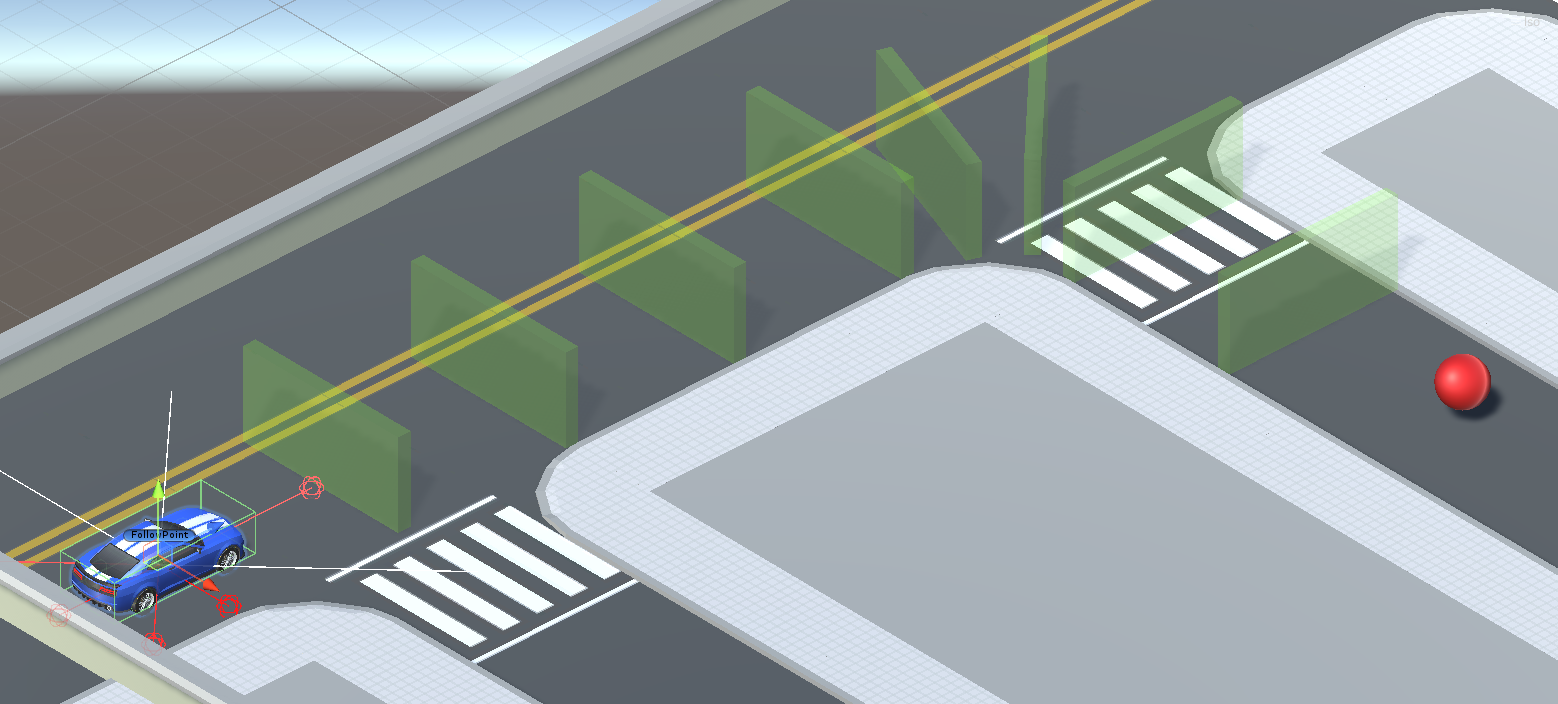
\includegraphics[scale=0.35]{figs/detalhe-rota.png}
    \caption{Rota vista de perspectiva isométrica, o agente posicionado a origem ao canto esquerdo, com os \textit{checkpoints} ao longo do percurso até o destino no canto direito.}
    \label{fig:route-view}
 \end{figure}

 \subsection{O agente}\label{agent-subsection}
 Para o aprendizado o veículo possui 8 sensores apontando para todas as direções uniformemente espaçadas, estes sensores são um \textit{component} do pacote \textbf{ML-agents} da Unity3D, são capazes de medir a distância dos objetos próximos ao veículo e também são capazes de distinguir quais são estes objetos. Estes sensores dentro do editor são representados por feixes que partem do centro do veículo, é possível configurar diversos atributos deles como a quantidade, o ângulo máximo de distância do primeiro ao último, o ângulo vertical (que indica se eles apontam para cima ou para baixo) e o tamanho da esfera, que nada mais é que a tolerância de colisão do sensor.

 \begin{figure}[h]
   \centering
   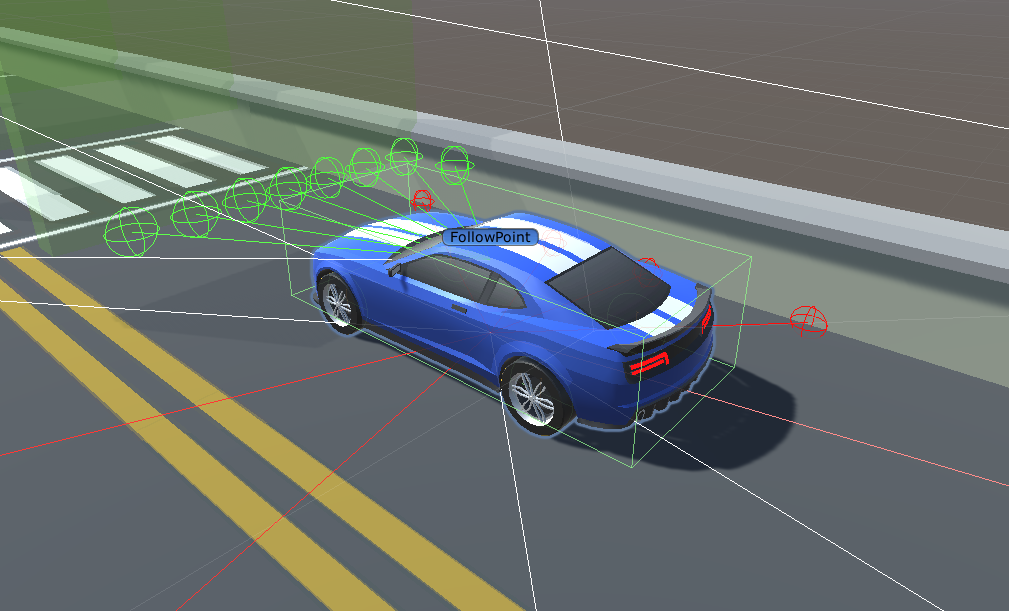
\includegraphics[scale=0.35]{figs/agente-raios-checkpoint.png}
    \caption{Exemplo do agente e seus raios perceptores, é possível ver 6 raios laterais se chocando com as calçadas ao lado, o raio frontal se chocando com o \textit{checkpoint}.}
    \label{fig:casting-rays}
 \end{figure}

 Além dos sensores, foi adicionado a velocidade do veículo a lista de observações do agente. Vale lembrar que o não foi implementado um recurso de imagem em um primeiro momento, ou seja, o veículo só enxerga através dos sensores e tem ciência de sua própria velocidade, ele é "cego" a qualquer outro elemento do ambiente que não esteja se choccando com o sensor.

 Quanto as ações que o agente pode fazer são apenas 3: acelerar, frear e direcionar as rodas a direita e a esquerda. A primeira e a última ação são chamadas ações contínuas, sendo assim um número que indica o nível de aceleração que o carro irá produzir, e no caso da direção da roda o quão direciona elas estão a esquerda ou direita. O ato de frear por outro lado é uma grandeza discreta, o veículo está ou não está freando.

\subsection{As recompensas}
Os eventos sujeitos a aplicação de recompensa/punição são os seguintes: o veículo chegar ao destino ($R_d$), o veículo atingir um checkpoint ($r_c$), colisão com a calçada ($p_c$), colisão com a parede($p_p$), tombar o veículo ($P_t$) e por fim a punição total por \textit{step} $P_{step}$. $R_d$, e $P_t$ são constantes e são eventos que definem o fim do episódio. Por outro lado, $r_c, p_c, p_p \text{ e } p_{step}$ serão aplicadas ao longo do episódio conforme os eventos ocorrerem, no caso do último o evento é o próprio \textit{step} e seu valor é $p_{step} = \frac{P_{step}}{N}$ sendo $N$ o número máximo de \textit{steps} por episódio.

Para o encerramento do episódio temos os seguintes cenários possíveis: o agente chega ao destino, o agente não chegar a tempo, o agente tombar o veículo. As recompensas estão no intervalo $[-1,1]$ e serão aplicadas da seguinte forma em cada cenário:

\begin{itemize}
   \item Chega ao destino: $R_T = R_d + R_c - P_c - P_p$
   \item Não chega a tempo: $R_T = R_c - P_{step} - P_c - P_p$
   \item Tomba o carro: $R_T = P_t \doteq -1$
\end{itemize}

Sendo $R_T$ a recompensa total do episódio, $R_c$, $P_c$ e $P_p$ representam a soma total de ocorrências de $r_c$, $p_c$ e $p_p$. Vale ressaltar que $R_d + R_c = 1$, isto quer dizer que se o veículo chegar ao destino sem se chocar com a calçada ou parede, terá a recompensa máxima, por outro lado $P_t = -1$, indicando que caso o veículo tombe, não interessa quantos checkpoints ele atingiu, a punição é máxima. Podemos interpretar o segundo cenário como: caso o veículo não chegue a tempo recebe uma recompensa pelo progresso ($R_c$) descontado com punição por tempo mais as punições por colisões. Sobre $r_c$, seu valor está sujeito ao trajeto do episódio, como eles possuem tamanho diferente, o valor a recompensa segue na forma $r_{c_x} \doteq \frac{R_c}{n_{c_x}}$, sendo $n_{c_x}$ a quantidade de checkpoints naquela rota $x$.

\subsection{O veículo}
Já vimos como funciona o agente agora vamos destrinchar como funciona a condução do \textit{GameObject} do veículo. O que foi explicado em \nameref{agent-subsection} se trata dos componentes que estão associados ao objeto do topo da hierarquia, o \textit{GameObject Car}. Abaixo do mesmo há dois objetos \textit{body} e \textit{spoiler} que são basicamente os \textit{meshes 3D} que dão o visual do veículo.

\begin{figure}[h]
   \centering
   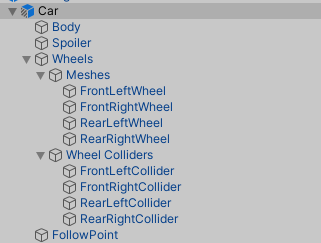
\includegraphics{figs/hierarquia-veiculo.png}
    \caption{Hierarquia dos \textit{GameObjects} que compõe o veículo.}
    \label{fig:vehicle-hierarchy}
\end{figure}

O terceiro objeto é \textit{Wheels} que agrega os objetos \textit{Meshes} e \textit{Wheel Colliders}, o primeiro é um conjunto dos \textit{meshes 3D} das rodas, o segundo agrupa os \textit{colliders} das mesmas. Estes últimos possuem um \textit{component} chamado \textit{Wheel Collider}, que é responsável pela física da roda (\citeonline{wheelcollider}) podendo configurar o raio, massa, amortecimento, etc. Todos os atributos estão com o valor padrão, exceto o raio que foi alinhado com o do \textit{mesh 3D}.

Para o controle do veículo foi adaptado um código fonte disponível em (\citeonline{PrismYoutube_2022}), neste código ele pega o input do usuário e atribui os mesmos a propriedades padrões dos \textit{colliders} das rodas dianteiras, o input "vertical" é aplicado ao torque do motor (\textit{motorTorque}), o "horizontal" ao ângulo de esterçamento do veículo (\textit{steeringAngle}, limitado a 30°). Ao frear é aplicado uma \textit{breakforce} nas quatro rodas. \textit{breakforce}, \textit{motorTorque} e \textit{steeringAngle} são todos propriedades do componente \textit{Wheel Collider} da Unity, basta associar os inputs do usuário a eles que a \textit{engine} da Unity3D lida com a física do veículo.

Para o projeto foi feito uma adaptação neste código-fonte, em vez de se aplicar o input do usuário, foi aplicado os valores que vem do \textit{actionBuffer}, que é um argumento de \textit{OnActionReceived()} a função que é responsável por tratar os dados das ações tomadas pelo agente. O \textit{actionBuffer} é um array que contém em cada elemento os valores da política naquele estado, isto é, o "input do agente".

O agente no projeto pode ser entendido como o conjunto de \textit{components} que fazem parte do GameObject pai, o "Car", seriam eles: behavior Parameters, o Car Agent, o Decision Requester e o Ray Perception sensor 3D. 

\section{Os algoritmos e hiper-parâmetros}\label{algoritmos}
Para executar o treino é necessário especificar para o \textbf{ml-agents} o algoritmo e suas configurações, para isso existe um arquivo \textbf{.yaml} que é responsável por isso. Abaixo, um exemplo seguido da explicação de cada parâmetro:

\begin{lstlisting}
behaviors:
   MoveToTarget:
      trainer_type: ppo
      max_steps: 9600000
      time_horizon: 64
      summary_freq: 60000
      keep_checkpoints: 16     
      checkpoint_interval: 600000
      hyperparameters:
         learning_rate: 1.0e-5
         batch_size: 1024
         buffer_size: 10240
         beta: 5.0e-2
         epsilon: 0.1
         lambd: 0.99
         num_epoch: 8
         learning_rate_schedule: linear
         beta_schedule: linear
         epsilon_schedule: linear
      network_settings:
         normalize: false
         hidden_units: 64
         num_layers: 2
      reward_signals:
         extrinsic:
            gamma: 0.99
            strength: 1.0
\end{lstlisting}

O arquivo começa com o \textbf{behaviors} que é uma lista de configurações dos comportamentos do agente, neste projeto haverá apenas um que é chamado \textbf{MoveToTarget}. Abaixo segue uma lista dos hiper-parâmetros mais relevantes, o texto aqui é em grande parte traduzido da documentação oficial do \textbf{ml-agents} (\citeonline{juliani2020}) com algumas remoções de informações não relevantes pra este projeto e com alguns adendos do autor caso necessário.

\begin{description}
   \item [trainer\_type:] O algoritmo que será usado, neste projeto serão PPO ou SAC
   \item [max\_steps:] O número máximo de passos(observações coletadas e ações tomadas pelo agente) tomados  no ambiente. No simulador a tarefa sempre será episódica, o tamanho do episódio pode variar nos ajustes, mas cada um possui em torno de 1200 \textit{steps}.
   \item [time\_horizon:] O número de \textit{steps} anteriores a ser coletado por agente para adicionar ao \textit{buffer} de experiência. Quando este limite é alcançado antes do fim de um episódio, um valor estimado é usado para prever a expectativa geral de recompensa a partir do estado atual do agente. Por isso, esse parâmetro varia entre menos enviesado mas com alta variância estimada (longo prazo) e mais enviesado mas com estimativa de menor variância (curto prazo). Em casos onde há frequente sinais de recompensas ou em episódios muito longos, um número menor pode ser mais ideal.
   \item [hyperparameters->learning\_rate:] Taxa inicial do salto a cada atualização do gradiente descendente. Este número geralmente deve diminuir com se o treino está instável e a recompensa com aumenta consistentemente.
   \item [hyperparameters->batch\_size:] O número de experiências coletadas para cada atualização do gradiente descendente. Em caso de usar ações contínuas ele deve estar na casa do milhares, caso contrário na casa das dezenas deve bastar.
   \item [hyperparameters->batch\_size:] Número de experiências a ser coletada antes de atualizar o modelo da política. Tipicamente, um buffer size maior corresponde a um treino mais estável. No caso do SAC este número deve ser milhares de vezes maior que um episódio típico, pois o algoritmo deve aprender de experiências velhas quanto mais novas.
   \item [hyperparameters->beta:] (somente PPO) força da regularização da entropia, que faz com que a política seja "mais aleatória". Isto garente que o agente explore apropriadamente o espaço da ação durante o treino. Aumenta-lo faz com que o agente tome mais ações aleatória. Isto deve ser ajustado de modo que o a entropia (medido pelo tensorboard) lentamente decresça conforme aumenta a recompensa. Se a entropia cair muito rápido aumente o \textbf{beta}, caso demore demais diminua-o.
   \item [hyperparameters->epsilon:] (somente PPO) Influencia no quão rapidamente a política pode evoluir durante o treino. Corresponde ao limite da divergência entre as velhas e novas políticas durante a atualização do gradiente descendente. Um valor menor leva a atualizações mais estáveis, mas deixa o processo de aprendizagem mais lento.
   \item [hyperparameters->lambd:] (somente PPO) parâmetro de regularização (lambda) usado quando calculado o estimador de valor generalizado (GAE (\citeonline{1506.02438})). Isto pode ser entendido em o quanto o agente depende no seu atual valor estimado quando atualizando o valor estimado. Valores baixos corresponde a apoiar-se mais no valor atual (alto viés/\textit{bias}) e valores elevados corresponde a confiar mais nas recompensas recebidas pelo ambiente (que pode causar alta variância). (geralmente varia de 0,9 a 0,99)
   \item [hyperparameters->num\_epoch:] (somente PPO) O número de passagens a fazer pelo buffer\_size quando otimizando gradiente descendente. Este deve crescer semelhante ao batch\_size. Diminui-lo tende a ter atualizações mais estáveis, aumentá-lo tem-se um treino mais lento. (geralmente varia entre 3 a 10)
   \item [hyperparameters->learning\_rate\_schedule:] Determina se o valor do learning\_rate muda durante o treino, os valores podem ser \textit{linear} ou \textit{constant}. Sendo o primeiro ele irá decair linearmente até zero quanto executar o \textit{max\_steps}. O segundo mantém o valor constante. É recomendado adotar \textit{linear} para PPO e o outro quando usar SAC.
   \item [hyperparameters->beta\_schedule:] (somente PPO) Similarmente ao acima mas para o \textbf{beta}. 
   \item [hyperparameters->epsilon\_schedule:] (somente PPO) Similarmente ao acima mas para o \textbf{epsilon}. 
   \item [hyperparameters->buffer\_init\_steps:] (somente SAC) Número de experiências a coletar no buffer antes de atualizar o modelo da política. Inicialmente o buffer é preenchido com ações aleatórias,o que é muito útil para exploração. Este número deve ser na casa de dezenas de vezes maior que um típico episódio.
   \item [hyperparameters->init\_entcoef:] (somente SAC) Corresponde a entropia inicial definida no começo do treino e é o quanto o agente deve explorar inicialmente. No SAC, o agente é incentivado a tomar decisões aleatorias a fim de explorar melhor o ambiente. O coeficiente de entropia é ajustado automaticamente para um valor alvo predefinido então o \textit{init\_entcoef} é apenas o valor inicial. Quanto maior o valor maior a exploração inicial. Para ações contínuas o típico valor está no invervalo 0,5-1,0, discreto em 0,05-0,5.
   \item [network\_settings->hidden\_units:] O número de nós em cada camada intermediária da rede neural totalmente conectada (valores típicos giram em torno de 32 a 512).
   \item [network\_settings->num\_layers:] O número de camadas intermediárias na rede neural (tipicamente tem valor de 1 a 3).
   \item [network\_settings->normalize:] Se normalização deve ser aplicada no vetor de observação. Esta normalização pode melhorar o treino em caso de tarefas que lidam com controles contínuos complexos, mas pode atrapalhar caso contrário.
\end{description}

\section{Desenvolvimento}\label{metodologia}
A análise e desenvolvimento do agente se dará tanto no treino quanto nos testes. O objetivo final é chegar a um agente que saiba percorrer todos os 17 trajetos de forma eficiente, para isso é preciso analisar as estatísticas produzidas pelo treino, saber se a política se aproximou suficientemente do comportamento ótimo de modo que cometa erros. Antes que se chegue a este nível é preciso que ele demonstre sucesso em treinos mais simples, então dividimos as etapas em 4 \textbf{desafios}. Os três primeiros serão em trajetos específicos, mas com níveis diferentes de dificuldade. O último será o treino o desafio geral, onde ele deve percorrer qualquer rota dada a ele.

Como foi dito na seção \nameref{sec:objetivos}, o estudo não propõe um modelo imutável, ao invés disso, é esperado que o agente evolua em diversas frentes: seus sensores, os métodos de treino, os algoritmos, o ambiente envolvido se torne mais realista, entre outros. Como será visto no Capítulo \ref{cap:resultados}, o agente e ambiente passou por mudanças a fim de cumprir as tarefas, estas alterações serão justificadas e compreendidas com os resultados dos treinos e testes.

\subsection{Treinamento e teste}
Tendo o \nameref{modelo} e \nameref{algoritmos} detalhados acima é preciso explicar o treinamento e teste. O treinamento é executado via linha de comando, é necessário ativar o ambiente Python, gerar um executável do simulador pelo editor da unity e ter um arquivo de configuração do algoritmo. Tendo estes três itens é possível executar o comando do ml-agents e por o agente em treino. Após o treino finalizar é gerado um arquivo \textbf{.onnx} que é política final do agente, a rede neural com os coeficientes gerados pelo algoritmo após o treino, o seu "cérebro". Finalmente podemos por o agente em teste, de volta ao editor da Unity3D, basta carregar o cérebro no agente e executar o teste, o veículo agora se move como a política traduz os estados em ações, definida no arquivo .onnx, sem qualquer input do usuário, e o mesmo deve estar agindo de acordo com os resultados do treino, seja ele um sucesso ou não.

Nos testes o agente deverá percorrer os mesmos trajetos, agora eles não serão aleatórios, ele percorrerá cada um três vezes. Como na lista de observações não inclui qualquer informação sobre qual trajeto ele está percorrendo no momento, o autor não viu necessidade de separar trajetos de treino e de teste, embora essa possibilidade posta em estudos futuros.

\subsubsection*{Estatísticas de treino}
Quando o treino é finalizado é armazenado diversas estatísticas que são exibidas pelo \textbf{tensorboard}. Nelas é possível ter uma visualização do desempenho do agente durante o treino e sua curva de aprendizado. As que serão analisadas e discutidas na próxima parte estão descritas na lista abaixo. Assimi como a listagem dos hiper-parâmetros essas definições são traduções diretas da documentação do ML-agents (\citeonline{juliani2020}).

\begin{description}
   \item [Cumulative Reward:] A mediana da recompensa acumulada no episódio do agente. Deve aumentar ao longo de um treino bem sucedido (Esta estatística possui dois gráficos, um de linha e outro histrograma)
   \item [Episode Length:] A duração mediana dos episódios (No caso deste projeto a duração deve diminuir ao longo do tempo, pois significa que o agente está realizando a tarefa mais eficientemente).
   \item [Entropy:] a entropia da política, isto é, o quão aleatório as decisões do modelo são. Deve decair durante um treino bem sucedido. Se decair muito rapidamente deve-se aumentar o valor do hiperparâmetro \textbf{beta}.
   \item [Extrinsic value estimate:] É a mediana do valor de todos os estados visitados pelo agente. Deve aumentar ao longo de um treinamento bem sucedido.
\end{description}

Os demais gráficos são o \textbf{beta}, \textbf{epsilon} e \textbf{learning\_rate} eles são basicamente o valor destes hiper-parâmetros ao longo do treino, dependendo se os \textit{schedules} deles forem constante ou linear, é esperado uma linha constante no primeiro caso ou uma queda do valor deles até zero caso linear.

\subsection{Estudo e análise}
Para cada desafio será avaliado o treino e teste. A análise do treino envolverá(além dos gráficos mencionados acima) o tempo que demorou para convergir, a mediana e desvio padrão da recompena final. Para o teste, teremos duas formas diferentes de avaliar. Para os três primeiros desafios, o agente deverá percorrer o percurso que treinou dez vezes, será avaliado pela recompensa média e a quantidade de vezes que chegou ao destino. Para o desafio geral, deverá percorrer todas as rotas três vezes, será avaliado da mesma forma, por rota e o consolidado total. O primeiro desafio será específico em uma rota retilínea, sem necessidade de fazer curvas. O segundo exigirá que o agente faça uma curva, será treinado em dois trajetos diferentes. O último antes do geral, exigirá mais de uma curva, será treinado em três trajetos distintos. Por fim o geral será treinado em todos os trajetos, de diferentes tamanhos e complexidade. Fora a análise quantitativa, haverá também uma análise mais subjetiva da condução do veículo.

\begin{table}[htpb]
   \centering
   \caption{Avaliação dos desafios. A coluna de rotas informa qual o \textit{GameObject} de rota que será treinado. A figura deles estará nos resultados.}
   \begin{tabular}{|l|p{3cm}|r|}
        \hline
        \small{Desafio}                   & \small{Rota(s)}                            & \small{Qtde. testes}     \\ \hline
         Específico: de trajeto fácil     & Path(2)                                    &      10                  \\ \hline
         Específico: de trajeto mediano   & Path(8)\newline Path(0)                    &      10 em cada rota     \\ \hline
         Específico: de trajeto difícil   & Path(3)\newline Path(5)\newline Path(6)    &      10 em cada rota     \\ \hline
         Geral                            & Todos                                      &      30 (3 em cada)      \\ \hline
   \end{tabular}
\end{table}

Aqui fica mais claro ao leitor o porquê o agente não é imutável, a cada desafio aumenta bastante a dificuldade da tarefa, exigindo uma calibragem mais sensível de hiper-parâmetros ou um sistema sensorial mais robusto. Neste capítulo foi ilustrado a versão mais básica do veículo e do ambiente mas no próximo, onde veremos sobre os resultados dos treinos e testes, será expostos as mudanças que precisaram ser feitas no modelo.

No teste de um desafio, o agente deverá completar ao menos 90\% dos trajetos e média de recompensa acima de 0,95 cumprir os requisitos antes de tentar o próximo. 

%%%%%
% considerar completar esta parte, adicionar perguntas que devem ser respondidas na análise
%%%%
 